% TikZ schematic: FFT Analysis Pipeline (standalone compile)
\documentclass[tikz,border=10pt]{standalone}
\usepackage{tikz}
\usetikzlibrary{positioning,arrows.meta,decorations.pathreplacing,calc}

\begin{document}
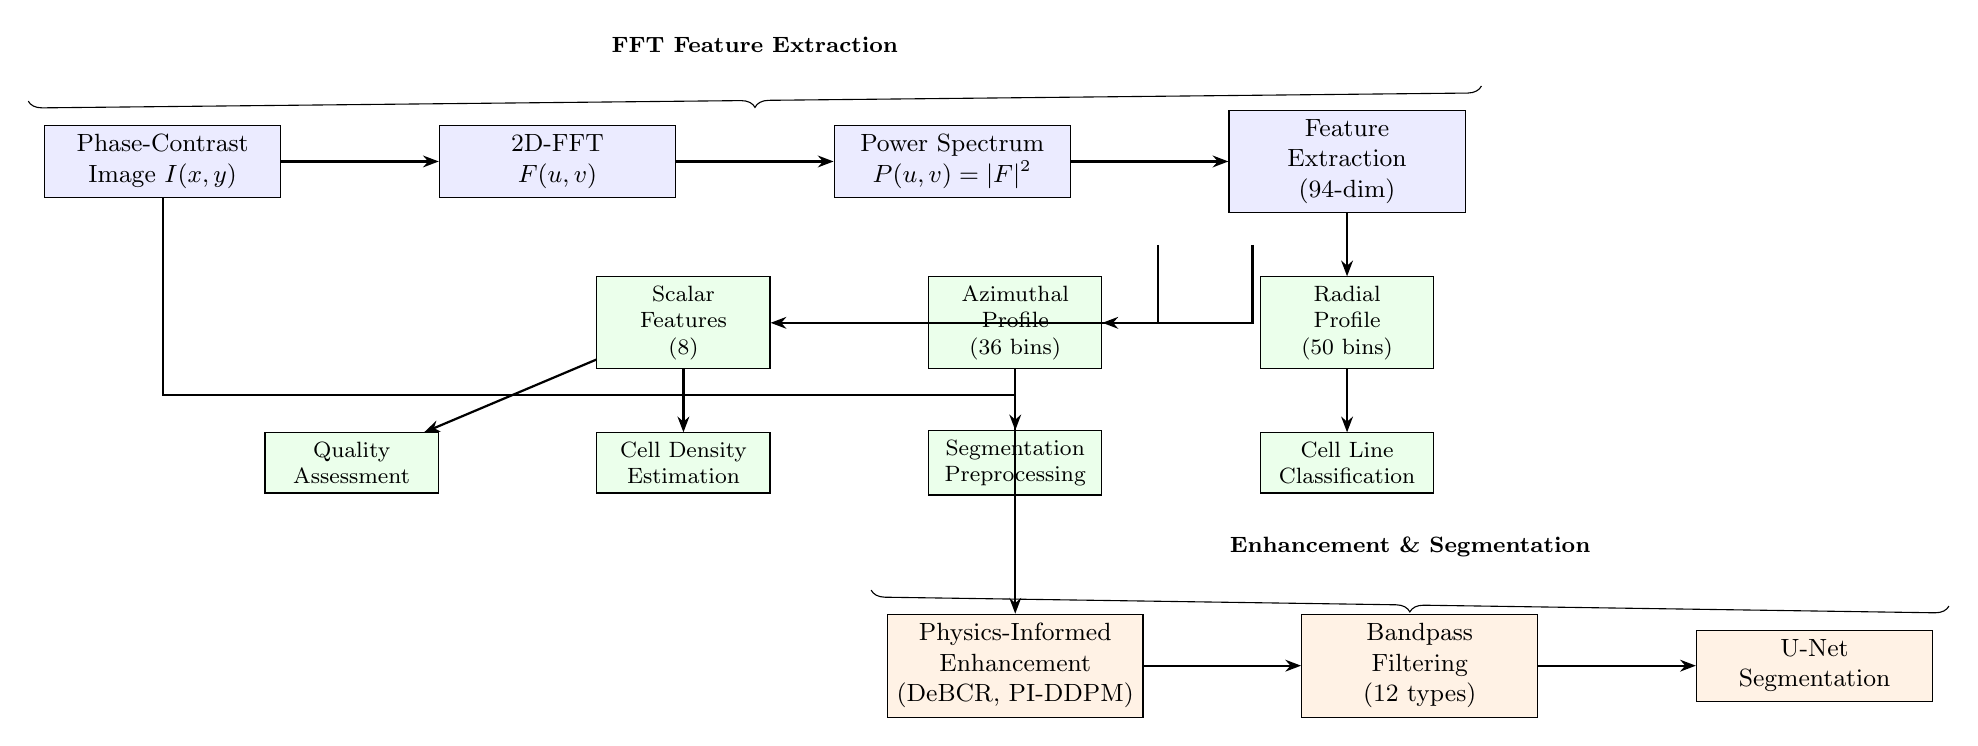
\begin{tikzpicture}[
    node distance=1.2cm and 2cm,
    block/.style={rectangle, draw, fill=blue!8, minimum width=3cm, minimum height=0.9cm, align=center, font=\small},
    smallblock/.style={rectangle, draw, fill=green!8, minimum width=2.2cm, minimum height=0.7cm, align=center, font=\footnotesize},
    arrow/.style={-{Stealth[length=2mm]}, thick},
    label/.style={font=\footnotesize, align=center}
]

% Row 1: Main pipeline
\node[block] (input) {Phase-Contrast\\Image $I(x,y)$};
\node[block, right=of input] (fft) {2D-FFT\\$F(u,v)$};
\node[block, right=of fft] (psd) {Power Spectrum\\$P(u,v)=|F|^2$};
\node[block, right=of psd] (feat) {Feature\\Extraction\\(94-dim)};

% Row 2: Analysis branches
\node[smallblock, below=0.8cm of feat] (radial) {Radial\\Profile\\(50 bins)};
\node[smallblock, left=of radial] (azimuth) {Azimuthal\\Profile\\(36 bins)};
\node[smallblock, left=of azimuth] (scalar) {Scalar\\Features\\(8)};

% Row 3: Applications
\node[smallblock, below=0.8cm of radial] (class) {Cell Line\\Classification};
\node[smallblock, left=of class] (seg) {Segmentation\\Preprocessing};
\node[smallblock, left=of seg] (density) {Cell Density\\Estimation};
\node[smallblock, left=of density] (quality) {Quality\\Assessment};

% Row 4: Enhancement branch
\node[block, below=1.5cm of seg, fill=orange!10] (enhance) {Physics-Informed\\Enhancement\\(DeBCR, PI-DDPM)};
\node[block, right=of enhance, fill=orange!10] (filter) {Bandpass\\Filtering\\(12 types)};
\node[block, right=of filter, fill=orange!10] (unet) {U-Net\\Segmentation};

% Arrows - main pipeline
\draw[arrow] (input) -- (fft);
\draw[arrow] (fft) -- (psd);
\draw[arrow] (psd) -- (feat);

% Arrows - features to branches
\draw[arrow] (feat.south) -- ++(0,-0.4) -| (radial);
\draw[arrow] (feat.south) ++(-1.2,-0.4) |- (azimuth);
\draw[arrow] (feat.south) ++(-2.4,-0.4) |- (scalar);

% Arrows - branches to applications
\draw[arrow] (scalar) -- (quality);
\draw[arrow] (scalar) -- (density);
\draw[arrow] (azimuth) -- (seg);
\draw[arrow] (radial) -- (class);

% Arrows - enhancement pipeline
\draw[arrow] (input.south) |- ++(0,-2.5) -| (enhance);
\draw[arrow] (enhance) -- (filter);
\draw[arrow] (filter) -- (unet);

% Brace labels
\draw[decorate, decoration={brace, amplitude=5pt, mirror}]
    ($(input.north west)+(-0.2,0.3)$) -- ($(feat.north east)+(0.2,0.3)$)
    node[midway, above=0.4cm, label] {\textbf{FFT Feature Extraction}};

\draw[decorate, decoration={brace, amplitude=5pt, mirror}]
    ($(enhance.north west)+(-0.2,0.3)$) -- ($(unet.north east)+(0.2,0.3)$)
    node[midway, above=0.4cm, label] {\textbf{Enhancement \& Segmentation}};

\end{tikzpicture}
\end{document}
